\documentclass{bjt}
% more options
% \documentclass[12pt]{bjt}
% by default 10pt, 16:9 aspect ratio

% \usepackage{hyperref}
% \hypersetup{colorlinks=true, linkcolor=., citecolor=., urlcolor=blue}

\usepackage{listings}
\lstdefinestyle{bjt}{
    language={python},
    basicstyle=\ttfamily\footnotesize,
    backgroundcolor=\color{gray!5},
    keywordstyle=\color{blue!75!black},
    commentstyle=\itshape\color{green!50!black},
    stringstyle=\color{red!70!black},
    showstringspaces=false,
    keepspaces=true,
    columns=fullflexible,
    frame=single,
    framerule=0.4pt,
    framesep=6pt,
    rulecolor=\color{black},
    breaklines=true,
    breakatwhitespace=true,
    numbers=left,
    numberstyle=\tiny\color{gray},
    numbersep=8pt,
    tabsize=2
}

\lstset{style=bjt}


% Presentation information
\newcommand{\Title}{Getting Started with the BJT Beamer Class}            % (EDIT HERE)
\newcommand{\Subtitle}{A Quick Introduction and User Guide}               % (EDIT HERE)
\newcommand{\AuthorName}{\textsc{Baijayanta}}                             % (EDIT HERE)
\newcommand{\EMail}{baijayantabhattacharyya2021@gmail.com}                % (EDIT HERE)
\newcommand{\InstituteName}{Department of Physics\\IIT Kharagpur\\\EMail} % (EDIT HERE)
\newcommand{\PresentationDate}{\today}                                    % (EDIT HERE)


% Beamer metadata
\title{\Title}               % (DO NOT EDIT HERE)
\subtitle{\Subtitle}         % (DO NOT EDIT HERE)
\author{\AuthorName}         % (DO NOT EDIT HERE)
\institute{\InstituteName}   % (DO NOT EDIT HERE)
\date{\PresentationDate}     % (DO NOT EDIT HERE)

\usepackage[edges]{forest}
\usepackage{adjustbox}
\usepackage{url}
%------------------------------------------------
\begin{document}

% make title frame
\maketitleframe

% make table of contents frame
\outlineframe

%================================================
\section{Introduction}
\begin{frame}{What is the BJT Class?}
The \texttt{bjt} class is a personal Beamer class built on top of the
\textbf{Metropolis} theme.

It provides

\begin{itemize}
    \item A modern scientific presentation style
    \item Modular theme architecture
    \item Custom colors and typography
    \item Physics-oriented shortcuts
    \item Custom title and background pages
    \item Backup slide management
    \item Bibliography support
    \item Easy customization
\end{itemize}
\end{frame}

%================================================
\section{Installation}

\begin{frame}{Directory Structure}

\begin{adjustbox}{max totalsize={\textwidth}{0.9\textheight}}
\begin{forest}
for tree={
    font=\small,
    grow'=0,
    child anchor=west,
    parent anchor=east,
    anchor=west,
    edge={-stealth},
    l sep=50pt,
    s sep=2pt,
}
[project
    [bjt
        [Theme files
            [backgrounds.sty]
            [backup.sty]
            [bjttheme.sty]
            [colors.sty]
            [commands.sty]
            [fonttheme.sty]
            [innertheme.sty]
            [outertheme.sty]
            [outlines.sty]
            [references.sty]
            [templates.sty]
            [thankyou.sty]
            [titlepage.sty]
        ]
    ]
    [bjt.cls]
    [{\color{blue}main.tex}]
    [bjt-ref.bib]
    [references.bib]
]
\end{forest}
\end{adjustbox}
\end{frame}
\slidebackground{}
%================================================
\section{Using the Class}

\begin{frame}[fragile]{Creating a Presentation}
Creating a presentation with the \texttt{bjt} class is straightforward.
\begin{adjustbox}{max totalsize={\textwidth}{0.7\textheight}}
\begin{lstlisting}
\documentclass{bjt}

% Presentation information
\newcommand{\Title}{Title}              % (EDIT HERE)
\newcommand{\Subtitle}{Subtitle}        % (EDIT HERE)
\newcommand{\AuthorName}{Name}          % (EDIT HERE)
\newcommand{\InstituteName}{University} % (EDIT HERE)
\newcommand{\PresentationDate}{\today}  % (EDIT HERE)

% Beamer metadata
\title{\Title}               % (DO NOT EDIT HERE)
\subtitle{\Subtitle}         % (DO NOT EDIT HERE)
\author{\AuthorName}         % (DO NOT EDIT HERE)
\institute{\InstituteName}   % (DO NOT EDIT HERE)
\date{\PresentationDate}     % (DO NOT EDIT HERE)

\begin{document}
\titlepage
\end{document}
\end{lstlisting}
\end{adjustbox}

The \texttt{bjt} class automatically loads the theme and the required
packages, so no additional setup is necessary.
\end{frame}

%\section{Frame Shortcuts}

% \begin{frame}[fragile]{Creating Frames Quickly}

% The command

% \begin{lstlisting}
% \myframe{Title}{Content}
% \end{lstlisting}

% creates

% \begin{lstlisting}
% \begin{frame}{Title}
% Content
% \end{frame}
% \end{lstlisting}

% Example:

% \begin{lstlisting}
% \myframe{Introduction}{
% This is a simple slide.
% }
% \end{lstlisting}

% \end{frame}

% \begin{frame}{Blank Slide}

% A clean slide without navigation elements:

% \begin{lstlisting}
% \blankframe
% \end{lstlisting}

% Useful for:
% \begin{itemize}
% \item Section separators
% \item Full-page figures
% \item Closing slides
% \end{itemize}
% \end{frame}

\section{Backgrounds}

\begin{frame}[fragile]{Title Background}
A custom title background can be added:
\begin{lstlisting}
\titlebackground[0.25]{image.jpg}
\maketitleframe
\end{lstlisting}
The first argument controls opacity. The opacity argument is optional.
\end{frame}

% set custom background to title
\titlebackground[0.2]{backgrounds/wallpaper.jpg}
\maketitleframe

\begin{frame}[fragile]{Slide Background}
Background images can also be applied globally:
\begin{lstlisting}
\slidebackground[0.15]{wallpaper.jpg}
\end{lstlisting}
The first argument controls opacity. The opacity argument is optional.

\vspace{1cm}

\begin{alertblock}{Note}
    Using \verb|\slidebackground{}| resets the previously applied background.
\end{alertblock}
\end{frame}

\slidebackground{backgrounds/wallpaper.jpg}
%\outlineframe[Today's Topics]

%================================================

\section{Typography}
\begin{frame}{Design Philosophy}

The class follows a modular structure.

\begin{block}{Core Theme}
Controls global appearance:
\begin{itemize}
    \item Colors
    \item Fonts
    \item Inner theme
    \item Outer theme
\end{itemize}
\end{block}

\vspace{-0.2cm}

\begin{exampleblock}{Templates}
Provides reusable components:
\begin{itemize}
    \item Title page
    \item Backgrounds
    \item References
    \item Backup slides
\end{itemize}
\end{exampleblock}

\end{frame}


\begin{frame}{Fonts}

This theme uses

\begin{itemize}
    \item Bookman as the text font
    \item EulerVM for mathematics
    \item Small-cap frame titles
    \item Serif font theme
\end{itemize}

Example:

\begin{align*}
    E &= mc^2\\[1ex]
    \int_0^\infty e^{-x^2}\,dx &= \frac{\sqrt{\pi}}{2}
\end{align*}

\end{frame}
\slidebackground{}
%================================================
\section{Blocks}

\begin{frame}{Block Environments}

\begin{block}{Normal Block}
This is the standard block.
\end{block}

\vspace{3mm}

\begin{alertblock}{Alert Block}
Use this for warnings or important remarks.
\end{alertblock}

\vspace{3mm}

\begin{exampleblock}{Example Block}
Useful for examples and exercises.
\end{exampleblock}

\end{frame}

%================================================
\section{Lists}

\begin{frame}{Itemized Lists}

The itemize environment uses customized checkmarks.
\begin{itemize}
    \item First item
    \item Second item
    \item Third item
\end{itemize}

\vspace{5mm}

Enumerations are unchanged.
\begin{enumerate}
    \item One
    \item Two
    \item Three
\end{enumerate}
\end{frame}

%================================================

\section{Figures}
\begin{frame}{Figures}

\begin{figure}
\centering
\includegraphics[width=0.3\textwidth]{example-image-c} % or latex-logo.jpg
\caption{LaTeX logo}
\end{figure}

Captions are automatically numbered.
\end{frame}


%================================================
\section{Tables}

\begin{frame}{Tables}

\centering

\begin{tabular}{lcc}
\toprule
Parameter & Value & Unit\\
\midrule
Mass & 1.2 & kg\\
Velocity & 15 & m/s\\
Time & 12 & s\\
\bottomrule
\end{tabular}

\end{frame}

%================================================

\section{Mathematics}

\begin{frame}{Displayed Mathematics}

The class loads the AMS packages automatically.

\vspace{0.4cm}

\[E = mc^2\]

\vspace{0.3cm}

\[\nabla\cdot\mathbf{E}=\frac{\rho}{\varepsilon_0}\]

\vspace{0.3cm}

\[G_{\mu\nu}+\Lambda g_{\mu\nu}=\frac{8\pi G}{c^4}T_{\mu\nu}\]

\end{frame}

% \begin{frame}{General Relativity Commands}

% Requires:

% % \begin{lstlisting}
% % \usepackage{tensor}
% % \end{lstlisting}


% Examples:

% %\[\Metric{\mu}{\nu}\]

% %\[\Christoffel{\mu}{\nu}{\rho}\]

% %\[\Einstein{\mu}{\nu}=\frac{8\pi G}{c^4}\StressEnergy{\mu}{\nu}\]

% \end{frame}

%================================================
\section{Customization}

\begin{frame}[fragile]{Changing Colors}

Modify

\begin{lstlisting}
bjt/colors.sty
\end{lstlisting}

Example:

\begin{lstlisting}
\setbeamercolor{structure}{fg=purple}

\setbeamercolor{progress bar}{fg=orange,bg=gray}
\end{lstlisting}

\end{frame}

%------------------------------------------------

\begin{frame}[fragile]{Changing Fonts}

Edit

\begin{lstlisting}
bjt/fonttheme.sty
\end{lstlisting}

For example,

\begin{lstlisting}
\RequirePackage{bookman}
\RequirePackage{eulervm}
\end{lstlisting}

Replace them with your preferred font packages.

\end{frame}

%------------------------------------------------

\begin{frame}[fragile]{Changing Blocks}

Modify

\begin{lstlisting}
bjt/innertheme.sty
\end{lstlisting}

For example,

\begin{lstlisting}
\setbeamertemplate{blocks}[rounded][shadow=true]
\end{lstlisting}

or

\begin{lstlisting}
\setbeamertemplate{itemize item}{\ensuremath{\checkmark}}
\end{lstlisting}

\end{frame}

%------------------------------------------------

\begin{frame}[fragile]{Changing the Footline}

Modify

\begin{lstlisting}
bjt/outertheme.sty
\end{lstlisting}

For example,

\begin{lstlisting}
\setbeamertemplate{footline}[frame number]
\end{lstlisting}

You can also adjust the progress bar thickness.

\end{frame}

\section{References}

\begin{frame}[fragile]{Bibliography}

References can be inserted automatically:

\begin{lstlisting}
\referencesframe{references.bib}
\end{lstlisting}

\begin{block}{Note}
    \verb|\referencesframe{references.bib}| sets the bib file. \verb|unsrt| is the default bibliography style. 
\end{block}

or with a custom style:

\begin{lstlisting}
\referencesframe[abbrvnat]{references.bib}
\end{lstlisting}

\end{frame}

%\section{Backup Slides}


% \begin{frame}[fragile]{Backup Management}

% Backup slides can be separated:

% \begin{lstlisting}
% \backupbegin

% \begin{frame}
% Extra material
% \end{frame}

% \backupend
% \end{lstlisting}


% The frame counter automatically returns
% to the main presentation.

% \end{frame}

%================================================
\begin{frame}{Summary}

The BJT Beamer Class provides

\begin{itemize}
    \item Modular theme architecture
    \item Modern Metropolis design
    \item Custom title pages
    \item Background control
    \item Physics-oriented commands
    \item Bibliography management
    \item Backup slide support
    \item Easy extension through packages
\end{itemize}


\vspace{5mm}

Designed for scientific presentations.
Happy \LaTeX{}ing!

\end{frame}

\thankyouframe

\appendix

\nocite{*}


\referencesframe[plainnat]{bjt-ref.bib}


\backupbegin

\section{Backup Slides}

\begin{frame}{Extra Derivation}
This is a backup slide.
\end{frame}

\tikzset{>=Latex}
\begin{frame}{Equivalence of Mass and Energy}

\begin{center}
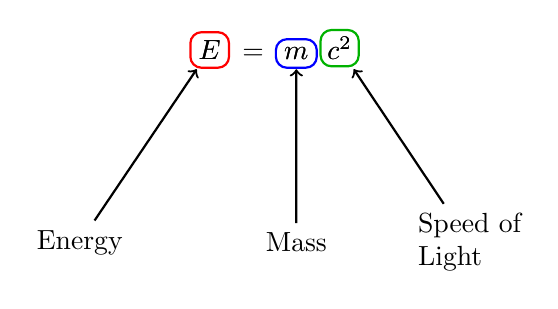
\begin{tikzpicture}[scale=1.1]

% Equation
\node[anchor = south] (E) at (-0.5,0) {$E$};
\node[anchor = south] (eq) at (0,0) {$=$};
\node[anchor = south] (m) at (0.5,0) {$m$};
\node[anchor = south] (c) at (1,0) {$c^2$};

%-----------------------------
% Step 2: Energy
%-----------------------------

\uncover<2>{
\node (energy) at (-2,-2) {Energy};
\draw[->,thick] (energy) -- (E);

% Highlight E
\node[draw=red,thick,rounded corners,inner sep=3pt] at (E) {$E$};}

%-----------------------------
% Step 3: Mass
%-----------------------------
\uncover<3>{\node (mass) at (0.5,-2) {Mass};
\draw[->,thick] (mass) -- (m);

% Highlight m
\node[draw=blue,thick,rounded corners,inner sep=3pt] at (m) {$m$};}


%-----------------------------
% Step 4: Speed of light
%-----------------------------
\uncover<4>{\node[align=left] (light) at (2.5,-2) {Speed of\\Light};
\draw[->,thick] (light) -- (c);

% Highlight c^2
\node[draw=green!70!black,thick,rounded corners,inner sep=2.5pt] at (c) {$c^2$};}

\end{tikzpicture}
\end{center}
\end{frame}

\begin{frame}{Source Code}
    This whole project is available at this link {\color{blue}\url{https://github.com/Baijayanta21/bjt-beamer-theme}}.
\end{frame}
\backupend

%------------------------------------------------
\end{document}